\section{Câu hỏi 3: Dự báo 7 ngày}

Trên Validation, Naive persistence có mean RMSE 5,535 m³/s, LightGBM delta 5,569 m³/s
và Seasonal Naive 365 65,57 m³/s. LightGBM không vượt Naive một cách ổn định; early
stopping chọn số vòng lặp rất nhỏ ở một số horizon, cho thấy mô hình gần như quay về
persistence. Vì vậy kết quả được báo cáo nguyên trạng, không tinh chỉnh thêm trên Test.

\begin{table}[H]
\centering
\caption{Chỉ số trên Test 2022--2023 (724 ngày gốc, 5.068 cặp dự báo)}
\label{tab:metrics}
\small
\setlength{\tabcolsep}{3pt}
\begin{tabular}{lrrrrr}
\toprule
Mô hình & mean RMSE & mean MAE & mean NSE & pooled RMSE & pooled NSE \\
\midrule
Naive persistence & 5{,}31 & 4{,}16 & 0{,}881 & 5{,}50 & 0{,}882 \\
Seasonal Naive 365 & 60{,}48 & 46{,}45 & -13{,}333 & 60{,}48 & -13{,}333 \\
LightGBM direct 7 (delta) & 5{,}33 & 4{,}17 & 0{,}881 & 5{,}52 & 0{,}881 \\
\bottomrule
\end{tabular}

\end{table}

Bảng~\ref{tab:metrics} cho thấy Naive persistence có mean RMSE \NaiveMeanRmse{} m³/s,
thấp hơn LightGBM \LgbmMeanRmse{} m³/s một chút. Seasonal Naive 365 rất kém
(\SeasonalMeanRmse{} m³/s), phù hợp với kết luận mùa vụ yếu ở Q1. Với LightGBM, D+1 có
RMSE 2,79 m³/s và NSE 0,970; D+7 có RMSE 7,10 m³/s và NSE 0,802. Naive cũng đi từ
2,79 m³/s ở D+1 lên 7,05 m³/s ở D+7. Sai số tăng theo horizon là hành vi hợp lý của
dự báo chuỗi thời gian.

\begin{figure}[H]
\centering
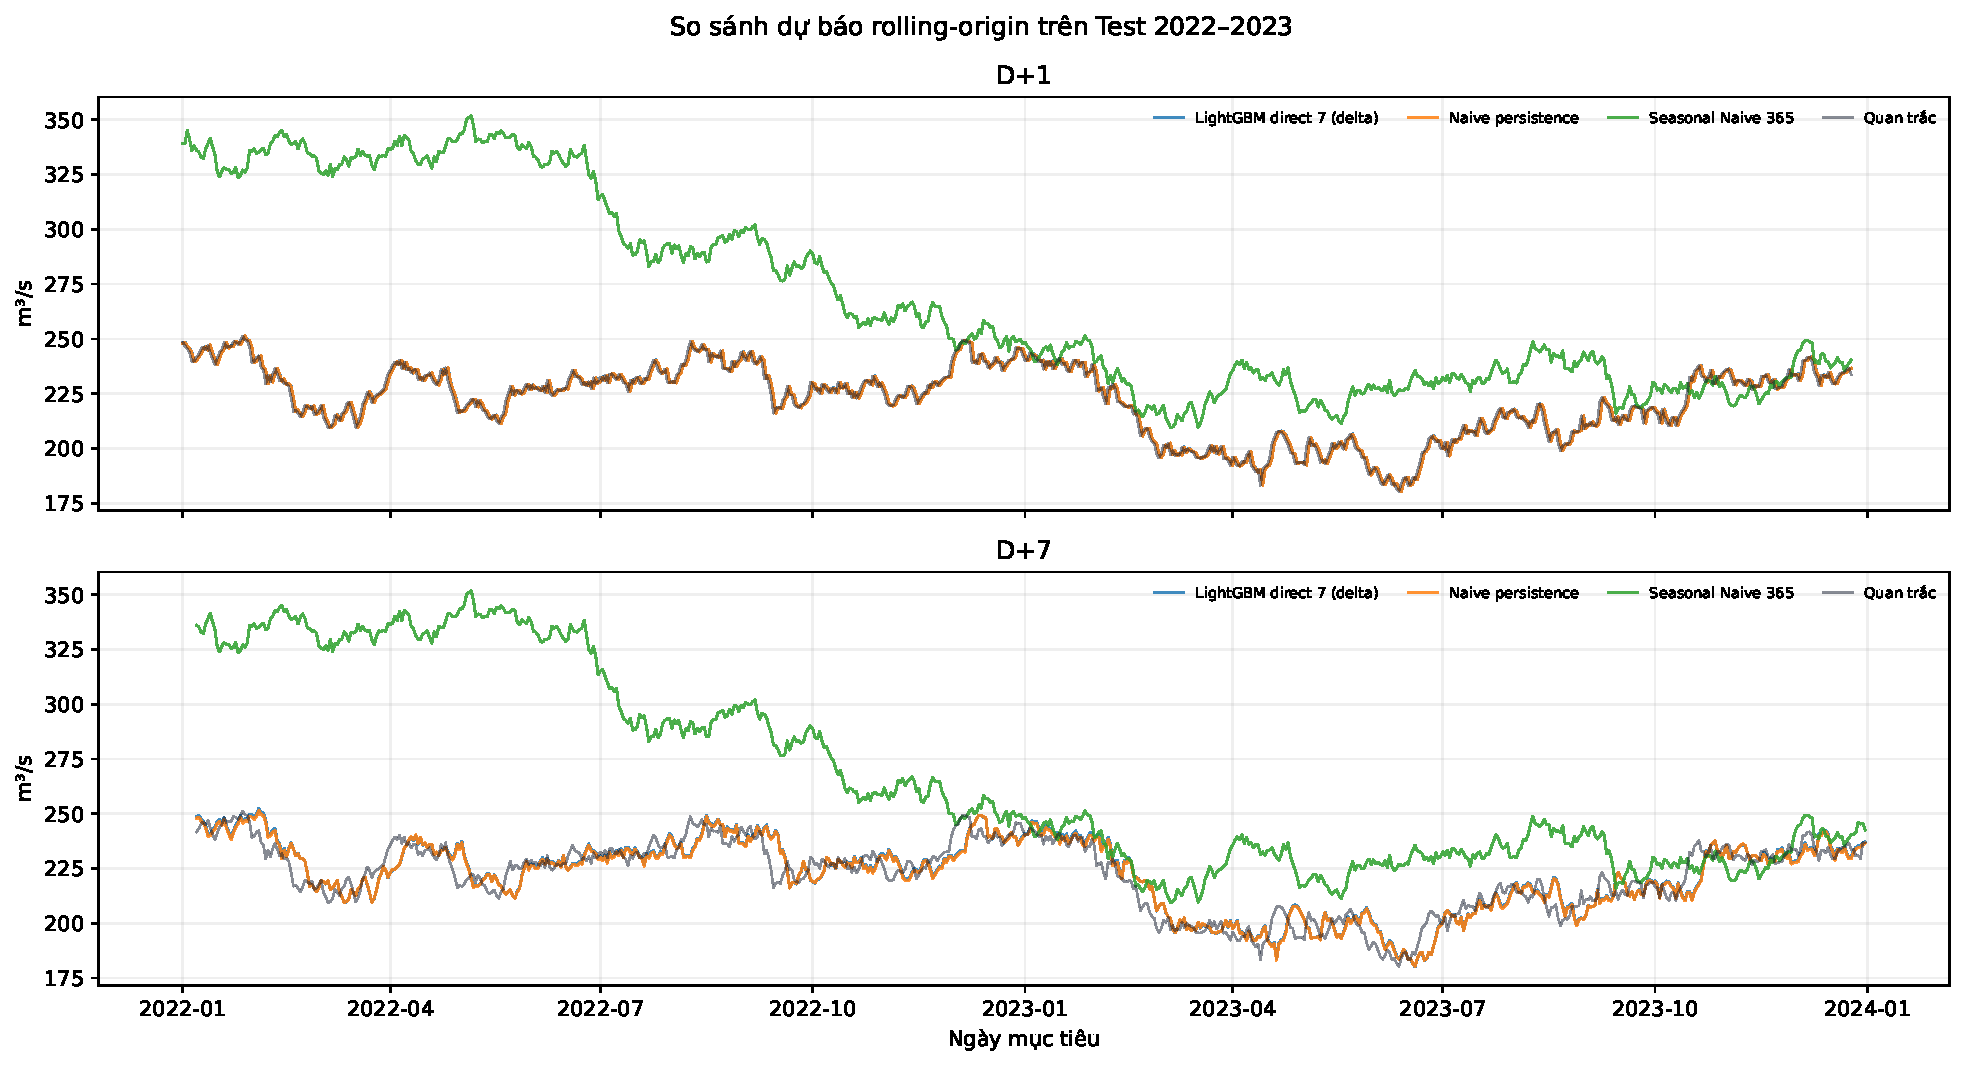
\includegraphics[width=0.84\linewidth]{figures/forecast_hydrograph.pdf}
\caption{Backtest 7 ngày: hai panel minh họa D+1 và D+7 với lịch sử, dự báo và giá trị
thực tế. Đường dự báo gần như bám mức persistence khi mô hình không tìm thấy tín hiệu
vượt trội.}
\label{fig:forecast}
\end{figure}

Kết quả này không có nghĩa LightGBM vô dụng. Mô hình vẫn học được cấu trúc phi tuyến
và đạt NSE cao, nhưng lợi thế so với persistence không ổn định trên Test. Với chuỗi
ngày có độ nhớt cao, baseline mạnh là đối thủ khó thay thế. Nếu mục tiêu là dự báo
vận hành, cần bổ sung biến ngoại sinh và đánh giá dài hạn hơn.
